%%%%%%%%%%%%%%%%%%%%%%%%%%%%%%%%%%%%%%%%%%%%%%%%%%%%%%%%%%%%%%%%%%
%%%%%%%% ICML 2013 EXAMPLE LATEX SUBMISSION FILE %%%%%%%%%%%%%%%%%
%%%%%%%%%%%%%%%%%%%%%%%%%%%%%%%%%%%%%%%%%%%%%%%%%%%%%%%%%%%%%%%%%%

% Use the following line _only_ if you're still using LaTeX 2.09.
%\documentstyle[icml2013,epsf,natbib]{article}
% If you rely on Latex2e packages, like most moden people use this:
\documentclass{article}

% For figures
\usepackage{graphicx} % more modern
%\usepackage{epsfig} % less modern
% \usepackage{subfigure}
\usepackage{subcaption}
\usepackage{multicol}

% For citations
\usepackage{natbib}

% For algorithms
\usepackage{algorithm}
\usepackage{algorithmic}

% For math
\usepackage{amsmath}

% As of 2011, we use the hyperref package to produce hyperlinks in the
% resulting PDF.  If this breaks your system, please commend out the
% following usepackage line and replace \usepackage{icml2013} with
% \usepackage[nohyperref]{icml2013} above.
\usepackage{hyperref}

% Packages hyperref and algorithmic misbehave sometimes.  We can fix
% this with the following command.
\newcommand{\theHalgorithm}{\arabic{algorithm}}

% Employ the following version of the ``usepackage'' statement for
% submitting the draft version of the paper for review.  This will set
% the note in the first column to ``Under review.  Do not distribute.''
\usepackage{icml2013}
% Employ this version of the ``usepackage'' statement after the paper has
% been accepted, when creating the final version.  This will set the
% note in the first column to ``Proceedings of the...''
% \usepackage[accepted]{icml2013}


% The \icmltitle you define below is probably too long as a header.
% Therefore, a short form for the running title is supplied here:
\icmltitlerunning{6.867: Homework 1}

\begin{document}

\twocolumn[
\icmltitle{6.867: Homework 1}

% % It is OKAY to include author information, even for blind
% % submissions: the style file will automatically remove it for you
% % unless you've provided the [accepted] option to the icml2013
% % package.
% \icmlauthor{Your Name}{email@yourdomain.edu}
% \icmladdress{Your Fantastic Institute,
%             314159 Pi St., Palo Alto, CA 94306 USA}
% \icmlauthor{Your CoAuthor's Name}{email@coauthordomain.edu}
% \icmladdress{Their Fantastic Institute,
%             27182 Exp St., Toronto, ON M6H 2T1 CANADA}

% You may provide any keywords that you
% find helpful for describing your paper; these are used to populate
% the "keywords" metadata in the PDF but will not be shown in the document
\icmlkeywords{boring formatting information, machine learning, ICML}

\vskip 0.3in
]

\section{Gradient descent}

We implemented a basic batch gradient descent procedure and applied it to minimize two different objective functions: the negative Gaussian function and the quadratic bowl function. Furthermore, after creating the implementations, we investigated how our choice of starting guess, step size, and convergence criterion/ threshold impacted our resulting solution. \\

Starting guess: \\

In general we saw that starting guess did not have much of an impact on our resulting solution. If the starting guess was farther away from the actual minimum, it simply took the algorithm a bit longer to actually converge. In the end though, the algorithm would converge for both of our objective functions. To the right you can see graphs with starting guesses of various orders of magnitude. \\

Step size: \\

Throughout our research, we discovered that step size actually had a pretty significant impact on our resulting solutions. For example, a step size that was too large would actually result in our gradient descent algorithm diverging instead of converging. This is illustrated in the figure on the right. As we can see, the algorithm oversteps on the first step which causes the norm of the new gradient to be larger than the original gradient norm. This then proceeds to compound at every step which ultimately causes the algorithm to diverge and go to infinity. \\

Convergence criterion/ threshold: \\

In addition to step size, the convergence criterion also has a pretty significant impact on the resulting solution. In general, we find that accuracy is inversely proportional to the convergence criterion while speed is directly proportional to the convergence criterion, which makes intuitive sense. Basically, with a large convergence criterion, the accuracy of the resulting solution is reduced while the algorithm runs to completion faster. On the other hand, with a smaller convergence criterion, the accuracy of the resulting solution is increased while the algorithm takes much longer to complete. \\

In order to make sure that our gradient functions were correct, we created a numerical gradient function so that we could validate the gradients at various points. To calculate the numerical gradients, we utilized the central difference approximation. For the quadratic bowl, it appears that no matter what the difference step was, the numerical gradient always equaled the true gradient. For the negative gaussian, we discovered that by making the difference step smaller, our numerical gradient gained accuracy and became closer to the true gradient. For example, at the point (0,0), the real gradient is [ -1.44009348e-06,   -1.44009348e-06]. The numerical gradient with a difference step of 100 is [ -1.14032986e-08 , -1.14032986e-08]. With a difference step of 10, the numerical gradient is [ -1.37214353e-06,  -1.37214353e-06]. With a difference step of 1, the numerical gradient is [ -1.43939760e-06,  -1.43939760e-06]. And lastly, with a difference step of 0.1, the numerical gradient is [ -1.44008652e-06,  -1.44008652e-06] (almost identical to the real gradient). From a mathematical perspective this makes intuitive sense because the very definition of a derivative is basically the numerical gradient as the difference step approaches 0. \\

In the next part of our research, we utilize two forms of gradient descent in order to try and minimize the following function: \\
$$J(\theta) = \Sigma_{i}(x^{(i)T}\theta - y^{i})^2$$ \\ 

Like before, we had to be really particular in the convergence criterion and step sizes we chose in order to ensure that the gradient descent converges. For batch gradient descent we chose an initial guess of all $0s$ with a step size of $10^{-6}$ and a convergence criterion of 1. This resulted in a $\theta$ that converged to  [  0.50832359  -2.33986133  -6.31150421   6.80803415  -1.06442692 6.66532056   3.39605963  -0.45908695 -12.94348103  15.73213395], which ultimately gave a minimum $J(\theta)$ of 8343.21291982. \\

In our stochastic gradient descent, we used the Robbins-Monro conditions in order to guarantee convergence. Specifically, we chose a $t$ value of $0.75$ and a $\gamma_{0}$ value of $10^{8}$. In terms of accuracy, it seems that the batch gradient descent is a bit more accurate. In terms of total number of evaluations, it also seems that the batch gradient has less.     
 
\label{submission}

As in the past few years, ICML will rely exclusively on
electronic formats for submission and review.


\subsection{Templates for Papers}


\section{Linear basis function regression}

We consider linear basis function regression as a method to benchmark the robustness of the gradient descent solution presented above. By using the closed-form maximum likelihood equation, we can calculate the maximum likelihood weight vector for our list of basis functions to approximate the data in the form of our basis. In this scenario, we are using data generated by $y(x) = \cos(\pi x) + 1.5 \cos(2 \pi x) + \epsilon(x)$, where $\epsilon(x)$ is some added noise to the dataset. Running linear regression on a simple polynomial basis of order $M$, where $\phi_0(x) = x^0$, $\phi_1(x) = x^1$, $\phi_2(x) = x^2$, ..., $\phi_M(x) = x^M$, we calculate the maximum likelihood weight vector by the following:
$$w_{ML} = (\Phi^T \Phi)^{-1} \Phi^T y$$
where $w_{ML}$ is the maximum likelihood weight vector and $\Phi$ is given by:
$$\Phi =
\begin{bmatrix}
  \phi_0(x_0)   & \phi_1(x_0)   & \phi_2(x_0)   & \dots   & \phi_M(x_0) \\
  \phi_0(x_1)   & \phi_1(x_1)   & \phi_2(x_1)   & \dots   & \phi_M(x_1) \\
  \vdots        & \vdots        & \vdots        & \ddots  & \vdots \\
  \phi_0(x_n)   & \phi_1(x_n)   & \phi_2(x_n)   & \dots   & \phi_M(x_n) \\
\end{bmatrix}
$$
Our choice of $M$, the degree of our polynomial basis, largely determines the fit of the regression to the data (Figure 2). More specifically, as small values of $M$, the polynomial basis cannot adequately capture all the data points. At higher values of $M$ however, overfitting occurs in which the weight vector performs well on the training data, but is not well generalized to new data. The value of $M$ therefore must be carefully considered in order to prevent too high variability in our generated regression polynomial. \\
\begin{figure}[width=\linewidth]
\centering
\begin{multicols}{2}
  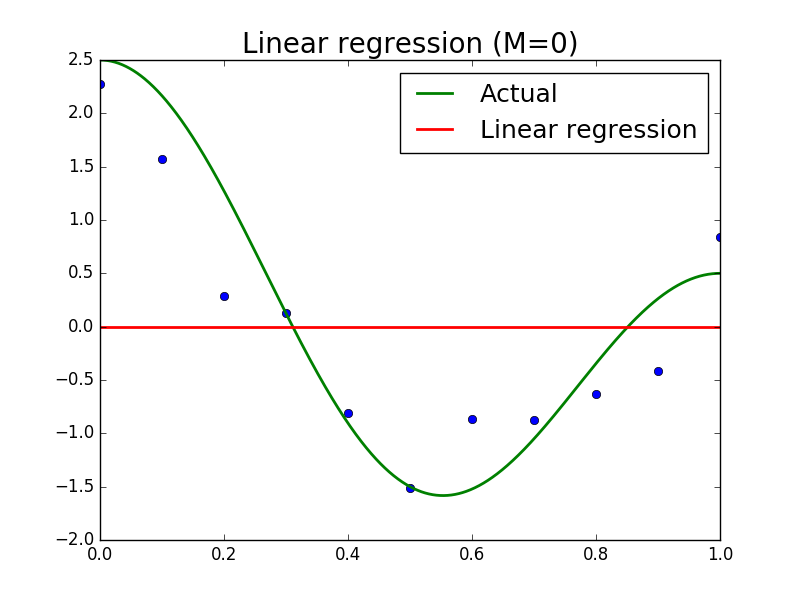
\includegraphics[width=1.2\linewidth]{code/P2/linear_regression,0.png}
  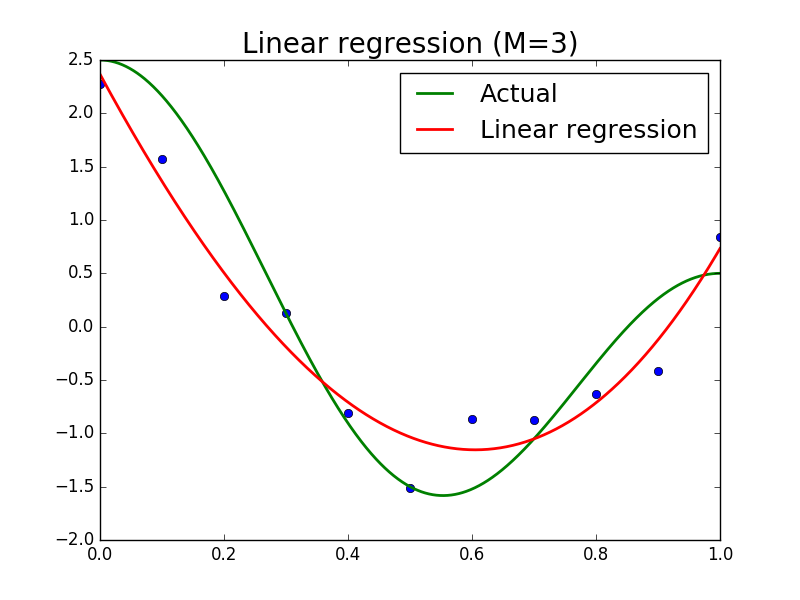
\includegraphics[width=1.2\linewidth]{code/P2/linear_regression,3.png}
  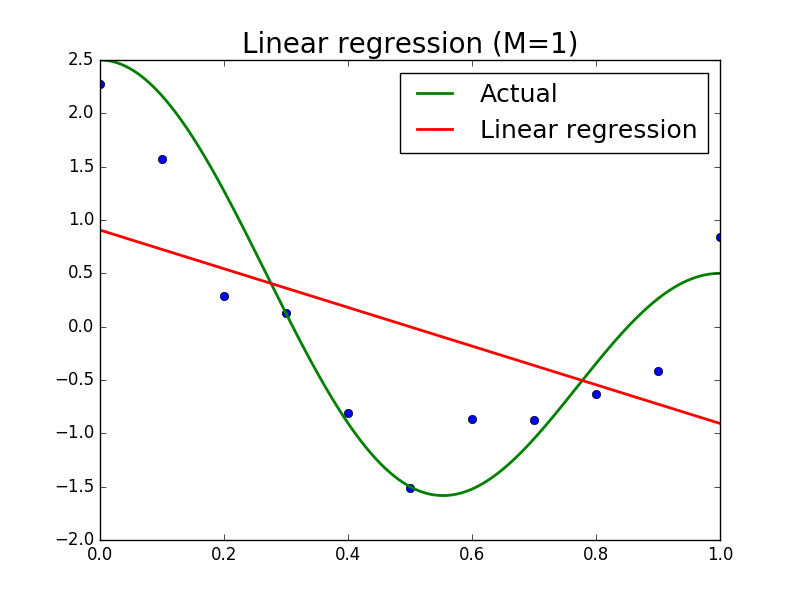
\includegraphics[width=1.2\linewidth]{code/P2/linear_regression,1.png}
  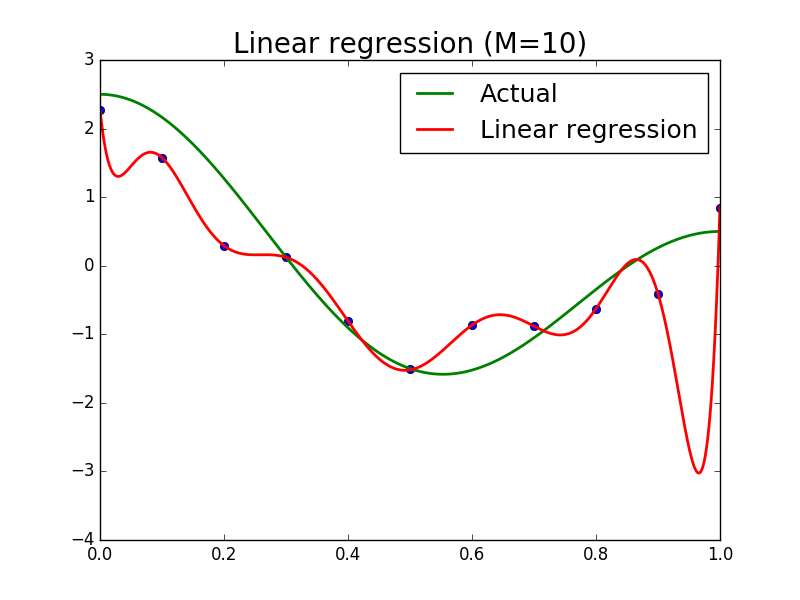
\includegraphics[width=1.2\linewidth]{code/P2/linear_regression,10.png}
\end{multicols}
\caption{Linear regression for varying values of M.}
\end{figure}

We can also instead choose our set of basis functions to be the set of cosine functions, where $\phi_1(x) = \cos(\pi x)$, $\phi_2(x) = \cos(2 \pi x)$, ..., $\phi_M(x) = \cos(M \pi x)$. This is again calculated for multiple values of $M$ and compared in Figure 3. Interestingly, even when we use the same family of basis functions as used to generate the initial data ($M=2$), due to the noise $\epsilon(x)$ added to the initial dataset, the maximum likelihood weight vector does not identically match the actual function used:
$$ w =
\begin{bmatrix}
  1 \\
  1.5
\end{bmatrix}$$
$$ w_{MLE} =
\begin{bmatrix}
  0.779 \\
  1.174
\end{bmatrix}$$

where $w$ is the actual weight vector and $w_{MLE}$ is the maximum likelihood estimated weight vector.
\begin{figure}[width=\linewidth]
\centering
\begin{multicols}{2}
  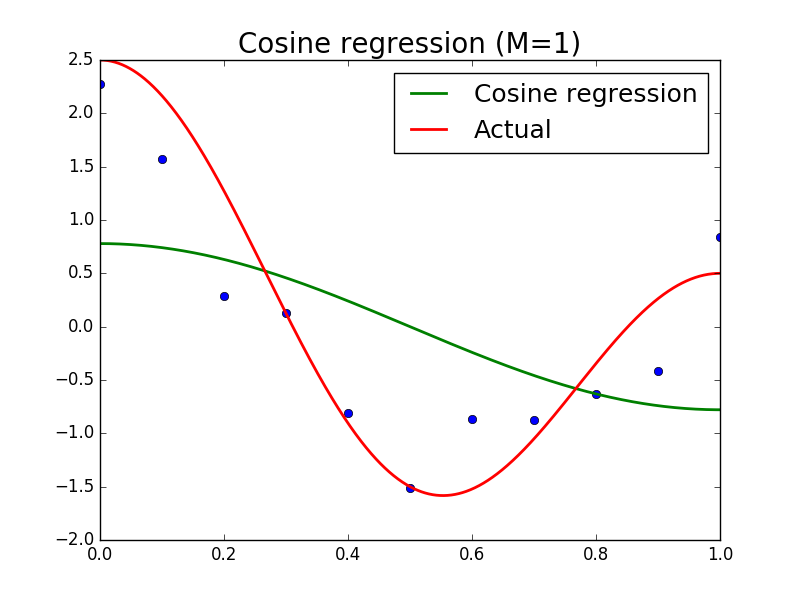
\includegraphics[width=1.2\linewidth]{code/P2/cosine_regression,1.png}
  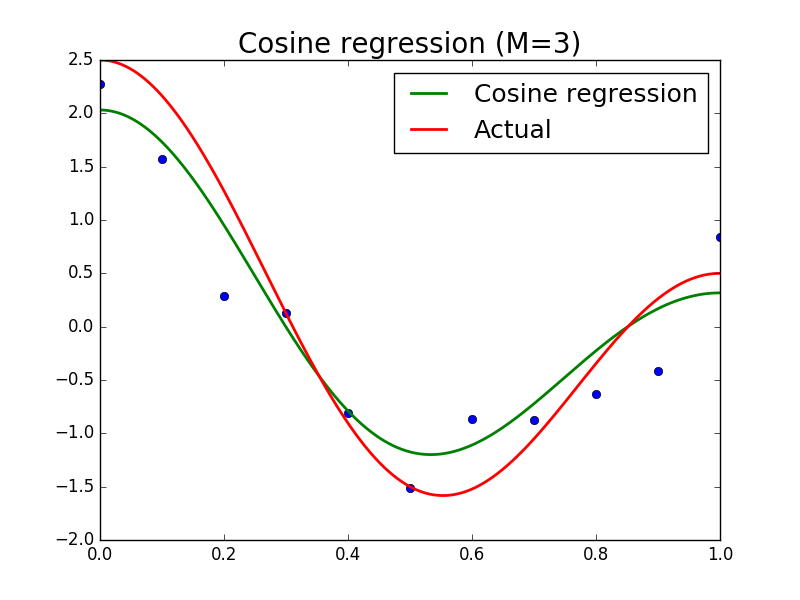
\includegraphics[width=1.2\linewidth]{code/P2/cosine_regression,3.png}
  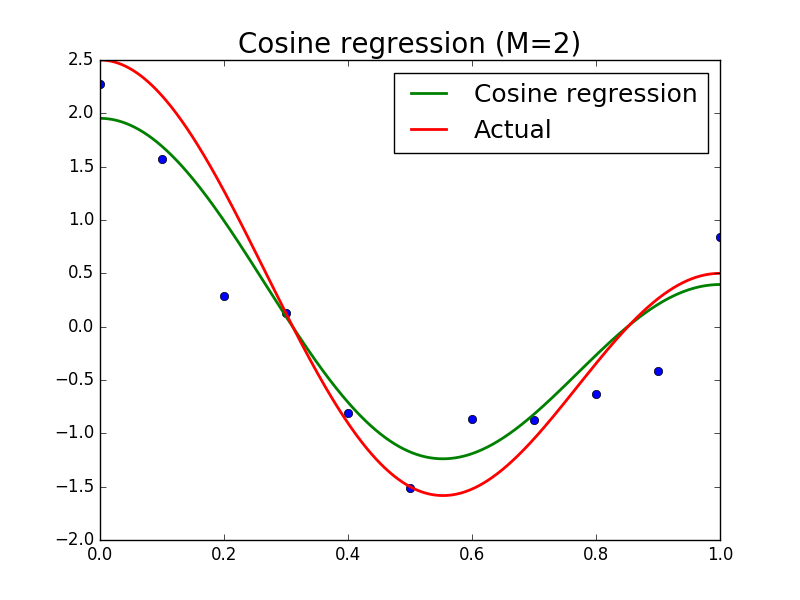
\includegraphics[width=1.2\linewidth]{code/P2/cosine_regression,2.png}
  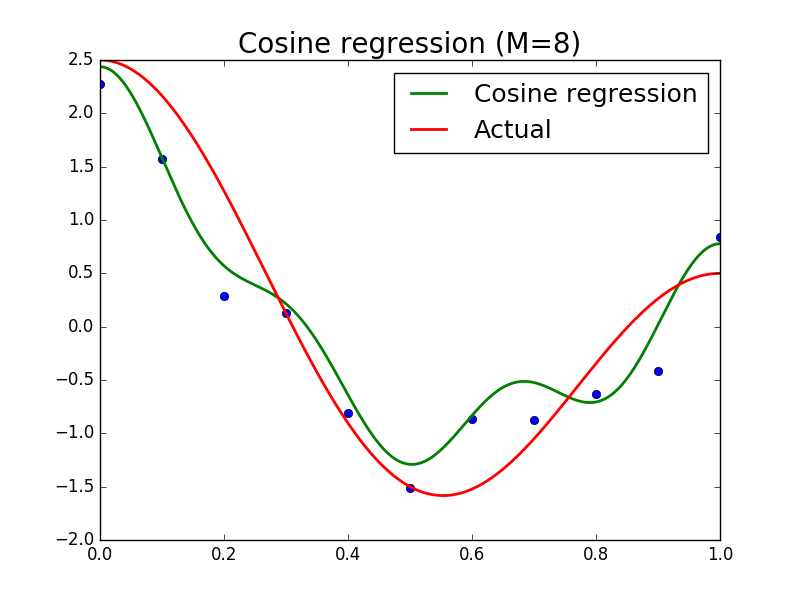
\includegraphics[width=1.2\linewidth]{code/P2/cosine_regression,8.png}
\end{multicols}
\caption{Linear regression for varying values of M.}
\end{figure}

\section{Ridge regression}

We can also instead choose our set of basis functions to be the set of cosine functions, where $\phi_1(x) = \cos(\pi x)$, $\phi_2(x) = \cos(2 \pi x)$, ..., $\phi_M(x) = \cos(M \pi x)$. Interestingly, even when we use the same family of basis functions as used to generate the initial data, due to the noise $\epsilon(x)$ added to our dataset, the maximum likelihood weight vector does not identically match the actual function used. This is visualized for varying values of $M$ in Figure 3.

We can also instead choose our set of basis functions to be the set of cosine functions, where $\phi_1(x) = \cos(\pi x)$, $\phi_2(x) = \cos(2 \pi x)$, ..., $\phi_M(x) = \cos(M \pi x)$. Interestingly, even when we use the same family of basis functions as used to generate the initial data, due to the noise $\epsilon(x)$ added to our dataset, the maximum likelihood weight vector does not identically match the actual function used. This is visualized for varying values of $M$ in Figure 3.

We can also instead choose our set of basis functions to be the set of cosine functions, where $\phi_1(x) = \cos(\pi x)$, $\phi_2(x) = \cos(2 \pi x)$, ..., $\phi_M(x) = \cos(M \pi x)$. Interestingly, even when we use the same family of basis functions as used to generate the initial data, due to the noise $\epsilon(x)$ added to our dataset, the maximum likelihood weight vector does not identically match the actual function used. This is visualized for varying values of $M$ in Figure 3.


\end{document}


% This document was modified from the file originally made available by
% Pat Langley and Andrea Danyluk for ICML-2K. This version was
% created by Lise Getoor and Tobias Scheffer, it was slightly modified
% from the 2010 version by Thorsten Joachims & Johannes Fuernkranz,
% slightly modified from the 2009 version by Kiri Wagstaff and
% Sam Roweis's 2008 version, which is slightly modified from
% Prasad Tadepalli's 2007 version which is a lightly
% changed version of the previous year's version by Andrew Moore,
% which was in turn edited from those of Kristian Kersting and
% Codrina Lauth. Alex Smola contributed to the algorithmic style files.
